%%%%%%%%%%%%%%%%%%%%%%%%
%
% $Autor: Keerti Belmane $
% $Datum: 2025-06-11 20:48:02Z $
% $Pfad: D:/BA_PROJECT/BA25-02-Time-Series/report/Contents/en/AppDevData.tex $
% $Version: 4621 $
%
% !TeX encoding = utf8
% !TeX root = Rename
%
%%%%%%%%%%%%%%%%%%%%%%%%
%%%%%%%%%%%%%%%%%%%%%%%%
%
% $Autor: Daanyaal Parvaize, Kreetika Mohanta, Keerti Belmane$
% $Datum: 2025-06-11 20:48:02Z $
% $Pfad: BA25-02-Time-Series/report/Contents/en/AppDevData.tex
% $Version: 4621 $
%
% !TeX encoding = utf8
% !TeX root = Rename
%
%%%%%%%%%%%%%%%%%%%%%%%%

\chapter{Documentation developer}

\section{Structure}
The dataset consists of 14 columns, each representing a specific attribute of Atlantic storms. The columns and their data types are as follows:

\begin{itemize}
	\item \texttt{Unnamed: 0} (integer): A sequential identifier or row number for each observation in the dataset, starting from 1 and incrementing for each new record.
	
	\item \texttt{name} (string): The official name assigned to the tropical cyclone (e.g., Amy, Blanche, Caroline), following the naming conventions for Atlantic storms.
	
	\item \texttt{year} (integer): The year in which the observation was recorded, ranging from 1975 onwards in this dataset.
	
	\item \texttt{month} (integer): The month of the observation, represented as a number from 1 (January) to 12 (December).
	
	\item \texttt{day} (integer): The day of the month when the observation was recorded.
	
	\item \texttt{hour} (integer): The hour of the day when the measurement was taken, using 24-hour format (0, 6, 12, 18), indicating measurements are typically taken at 6-hour intervals.
	
	\item \texttt{lat} (float): The latitude coordinate of the storm's center, measured in degrees. Positive values represent locations north of the equator.
	
	\item \texttt{long} (float): The longitude coordinate of the storm's center, measured in degrees. Negative values represent locations west of the prime meridian (in the western hemisphere).
	
	\item \texttt{status} (string): The classification of the storm system, such as "tropical depression," "tropical storm," "hurricane," "extratropical," or "subtropical storm/depression."
	
	\item \texttt{category} (float): The Saffir-Simpson Hurricane Wind Scale category, ranging from 1-5 for hurricanes, with NA for non-hurricane systems. Higher values indicate more intense hurricanes.
	
	\item \texttt{wind\_speed} (integer): The maximum sustained wind speed associated with the storm, measured in knots (nautical miles per hour).
	
	\item \texttt{pressure} (integer): The minimum central atmospheric pressure of the storm system, measured in millibars (mb). Lower values indicate more intense storms.
	
	\item \texttt{tropicalstorm\_force\_diameter} (float): The diameter of the area experiencing tropical storm force winds greater or equal to 34 knots), likely measured in nautical miles. Contains many NA values.
	
	\item \texttt{hurricane\_force\_diameter} (float): The diameter of the area experiencing hurricane force winds ( greater or equal to 64 knots), likely measured in nautical miles. Contains many NA values.
\end{itemize}

\begin{table}[htbp]
	\centering
	\caption{Summary of Atlantic Storm Dataset Variables}
	\begin{tabular}{|p{4cm}|p{3cm}|p{7cm}|}
		\hline
		\textbf{Variable} & \textbf{Data Type} & \textbf{Description} \\
		\hline
		Unnamed: 0 & Integer & Sequential row identifier \\
		\hline
		name & String & Storm name (e.g., Amy, Blanche) \\
		\hline
		year & Integer & Year of observation \\
		\hline
		month & Integer & Month of observation (1-12) \\
		\hline
		day & Integer & Day of observation \\
		\hline
		hour & Integer & Hour of observation (0, 6, 12, 18) \\
		\hline
		lat & Float & Latitude in degrees (+ = North) \\
		\hline
		long & Float & Longitude in degrees (- = West) \\
		\hline
		status & String & Storm classification (tropical depression, tropical storm, hurricane, etc.) \\
		\hline
		category & Float & Saffir-Simpson Hurricane Scale (1-5, NA for non-hurricanes) \\
		\hline
		wind\_speed & Integer & Maximum sustained wind speed (knots) \\
		\hline
		pressure & Integer & Minimum central pressure (millibars) \\
		\hline
		tropicalstorm\_force\_diameter & Float & Diameter of tropical storm force winds (nautical miles) \\
		\hline
		hurricane\_force\_diameter & Float & Diameter of hurricane force winds (nautical miles) \\
		\hline
	\end{tabular}
\end{table}

\newpage
\section{Size}
\begin{itemize}
	\item Number of rows (records): 19,066
	\item Number of columns (features): 14
	\item File size: 1,263,886 bytes (approximately 1.26 MB)
\end{itemize}

\section{Format}
The data is stored in \textbf{CSV (Comma-Separated Values)} format, which is a plain text format commonly used for tabular data storage and exchange.

\section{Anomalies}
\begin{itemize}
	\item \textbf{Missing Values:}
	\begin{itemize}
		\item \texttt{category}: 14,382 missing entries
		\item \texttt{tropicalstorm\_force\_diameter}: 9,512 missing entries
		\item \texttt{hurricane\_force\_diameter}: 9,512 missing entries
	\end{itemize}
	\item \textbf{Outliers:} No wind speed values exceed 200 knots, so no extreme outliers were detected in the \texttt{wind\_speed} column.
\end{itemize}

\subsection{Important Columns}

To build effective forecasting models for hurricane intensity, the following columns are especially important from the \texttt{storms.csv} dataset. These variables serve as the foundation for both statistical and deep learning models like ARIMA and LSTM.

\begin{itemize}
	\item \textbf{Date:} Timestamp of observation, essential for time series ordering.
	\item \textbf{Wind:} Maximum sustained wind speed — the target variable for prediction.
	\item \textbf{Pressure:} Atmospheric pressure, often inversely related to wind intensity.
	\item \textbf{Latitude and Longitude:} Geographical position of the storm, useful for spatial features in LSTM.
	\item \textbf{Status:} Storm classification (e.g., Tropical Storm, Hurricane), which can enhance feature modeling.
\end{itemize}

\begin{figure}[h]
	\centering
	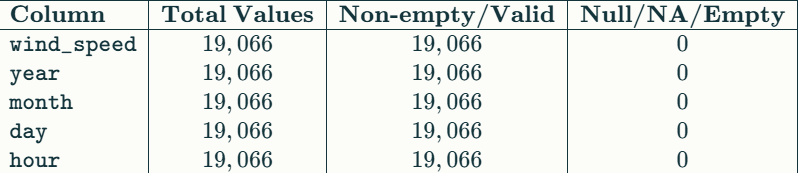
\includegraphics[width=0.8\textwidth]{Images/ImportantColumns.png}
	\caption{Important Columns for Hurricane Intensity Prediction}
	\label{fig:important-columns}
\end{figure}




\section{Origin}
The Atlantic hurricane dataset (HURDAT2) is maintained by NOAA and provides comprehensive best-track data for all known tropical and subtropical cyclones in the Atlantic basin\cite{noaa2021hurdat2}.
